\subsubsection{Fungsionalitas pada Domain Company}

Pengujian dengan ID P01 dilakukan dengan skenario yaitu admin berhasil membuat \textit{company} baru dengan nama \textit{cluster} yang tersedia pada sistem. Tersedia artinya konfigurasi kubernetes \textit{cluster} terdapat pada kubernetes \textit{config server}. Daftar \textit{cluster name} yang tersedia dapat dilihat pada gambar \ref{fig:list-cluster-tersedia}. Admin akan membuat request dengan Postman kepada \textit{server} dengan request seperti berikut.

\begin{enumerate}
  \item Mengisi \textit{field name} dengan nilai "new company"
  \item Mengisi \textit{field cluster\textunderscore name} dengan nilai "kind-testing-cluster-two-nodes"
\end{enumerate}

\textit{Request} dibuat dengan membuat request menggunakan Postman pada url /admin-api/v1/companies dengan metode POST. \textit{Request dan Response} dapat dilihat pada gambar \ref{fig:pengujian-p01}

\begin{figure}[ht]
  \centering
  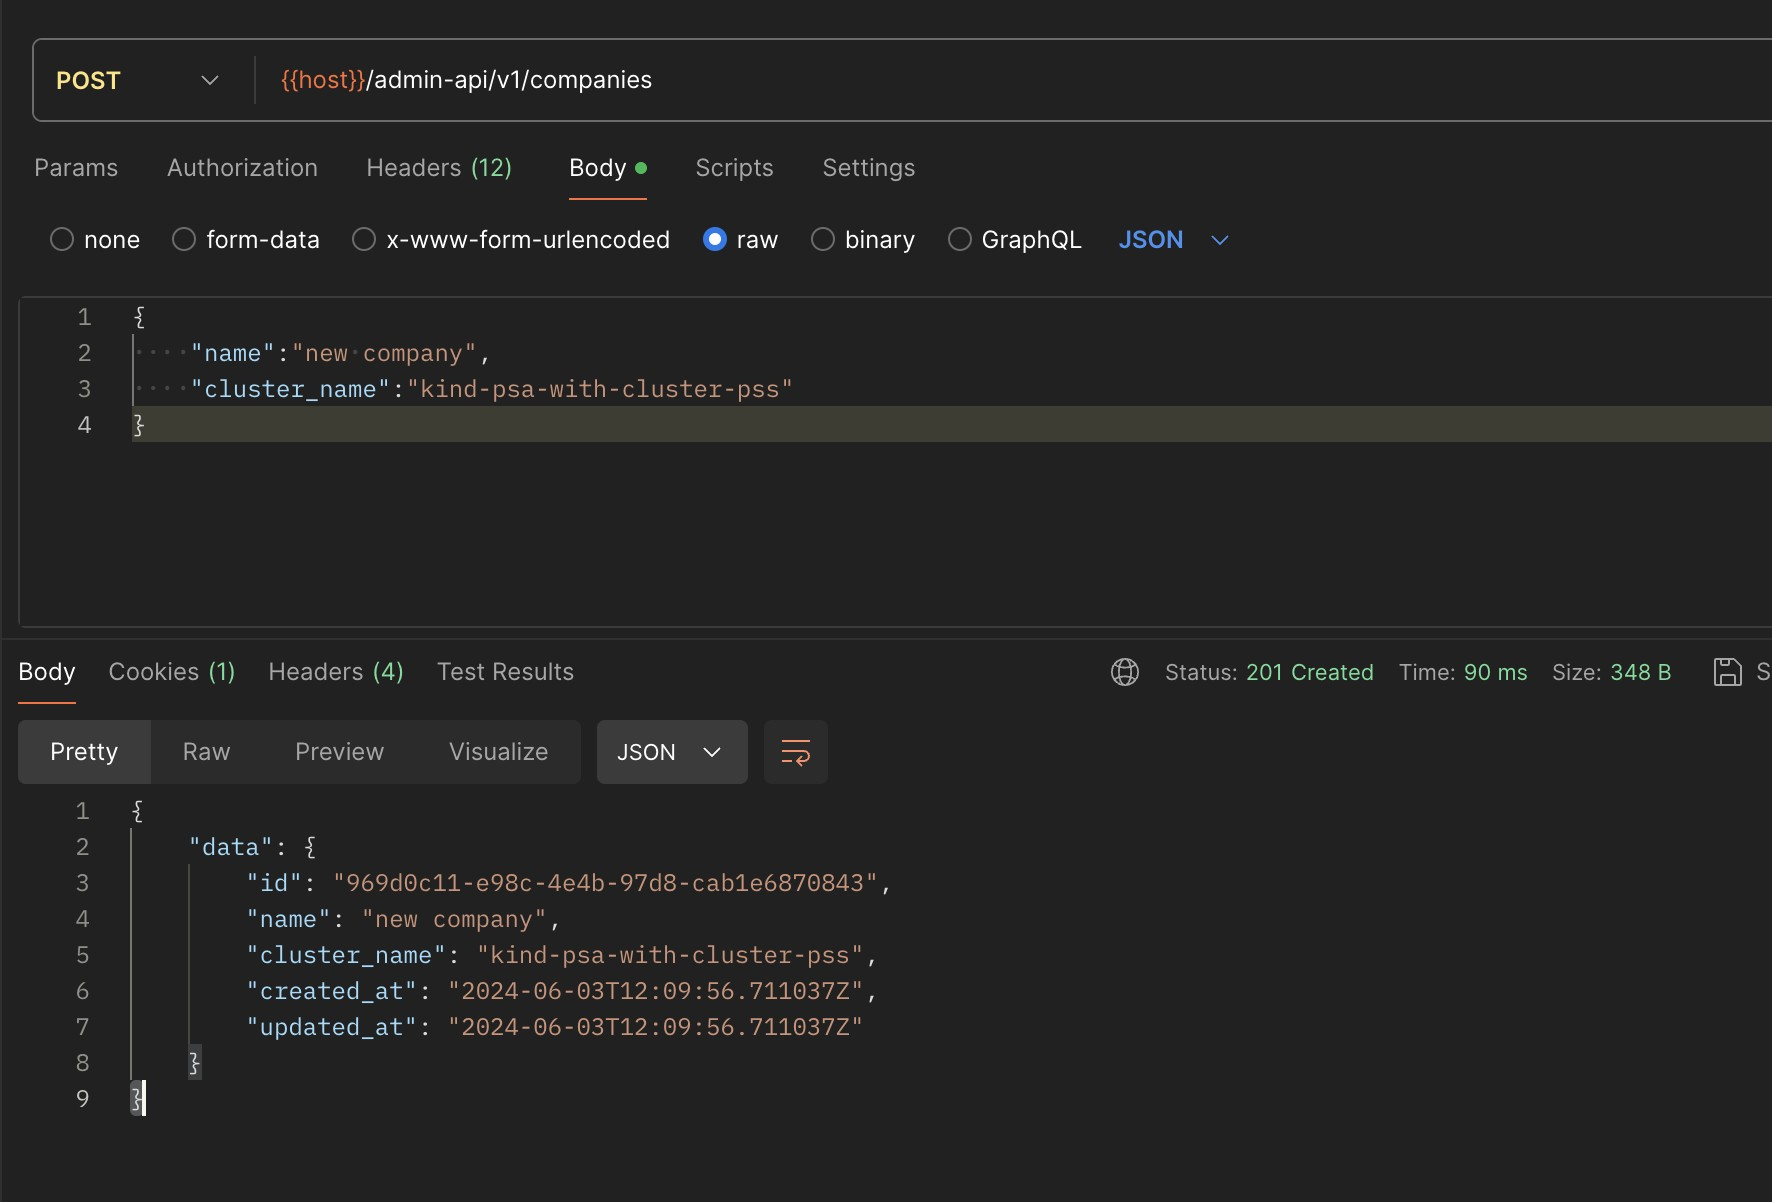
\includegraphics[width=0.8\textwidth]{resources/chapter-4/pengujian/p01.jpg}
  \caption{\textit{Request dan Response Pengujian} P01}
  \label{fig:pengujian-p01}
\end{figure}

Pengujian dengan ID P02 dilakukan dengan skenario yaitu admin tidak berhasil membuat \textit{company} karena nama cluster yang tidak tersedia pada server. Tersedia berarti, konfigurasi kubernetes cluster terdapat pada kubernetes \textit{config server} Admin akan membuat request dengan Postman kepada server dengan request seperti berikut.

\begin{enumerate}
  \item Mengisi \textit{field name} dengan nilai "new company"
  \item Mengisi \textit{field cluster\textunderscore name} dengan nilai "kind-testing-cluster-two-node"
\end{enumerate}

\textit{Request} dibuat dengan membuat request menggunakan Postman pada url /admin-api/v1/companies dengan metode POST. \textit{request dan response} dapat dilihat pada gambar

\begin{figure}[ht]
  \centering
  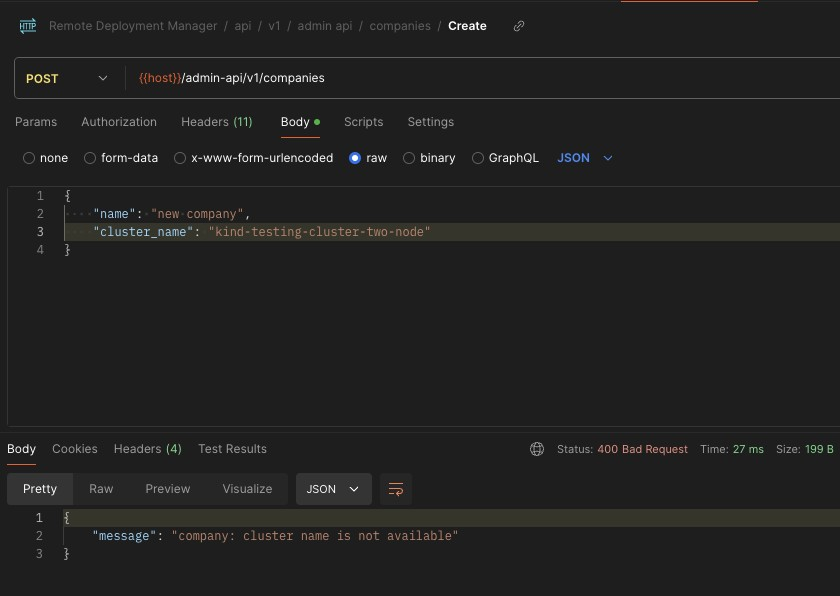
\includegraphics[width=0.8\textwidth]{resources/chapter-4/pengujian/p02.jpg}
  \caption{\textit{Request dan Response Pengujian} P02}
  \label{fig:pengujian-p02}
\end{figure}

Pengujian dengan ID P03 dilakukan dengan skenario yaitu admin ingin mendapatkan seluruh \textit{company} yang terdaftar pada sistem. Admin akan membuat GET request dengan Postman ke url /admin-api/v1/companies. \textit{Response} balikan dari \textit{request} dapat dilihat pada gambar \ref{fig:pengujian-p03}

\begin{figure}[ht]
  \centering
  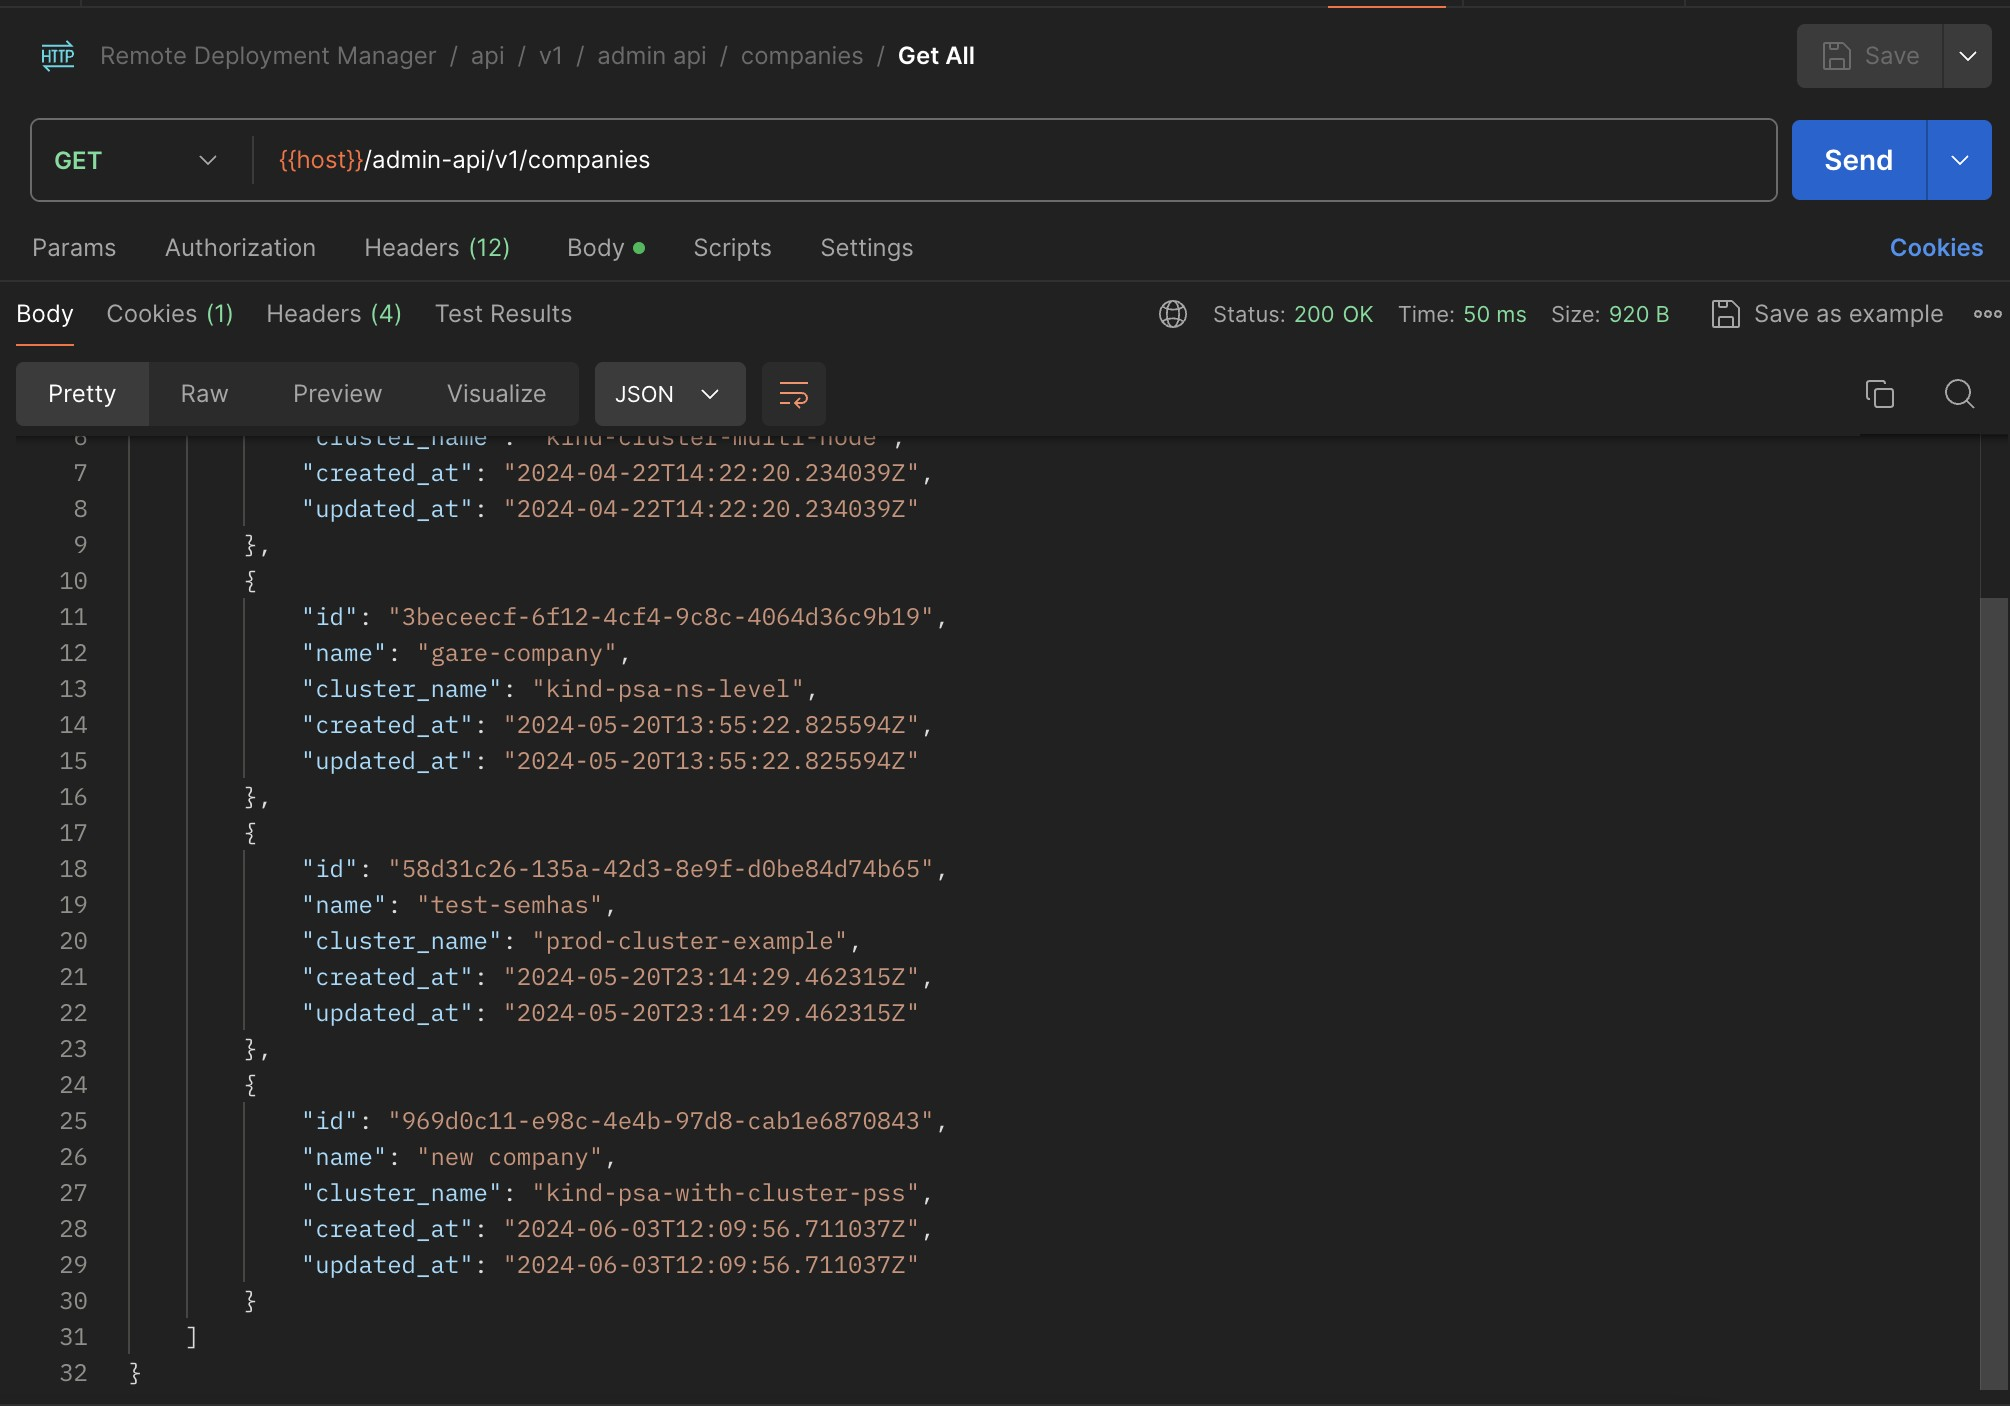
\includegraphics[width=0.8\textwidth]{resources/chapter-4/pengujian/p03.jpg}
  \caption{\textit{Request dan Response Pengujian} P03}
  \label{fig:pengujian-p03}
\end{figure}

Pengujian dengan ID P04 dilakukan dengan skenario yaitu admin ingin menghapus \textit{company} dengan id tertentu dari daftar \textit{company} pada sistem. Admin akan membuat DELETE request dengan Postman ke url /admin-api/v1/companies/:id. Untuk itu dibuat sebuah \textit{company} baru dengan spesifikasi sebagai berikut.

\begin{enumerate}
  \item Mengisi \textit{field name} dengan nilai "new company"
  \item Mengisi \textit{field cluster\textunderscore name} dengan nilai "kind-psa-with-cluster-pss"
\end{enumerate}

Hasil pembuatan \textit{company} dapat dilihat pada gambar \ref{fig:pengujian-p04-1}

\begin{figure}[ht]
  \centering
  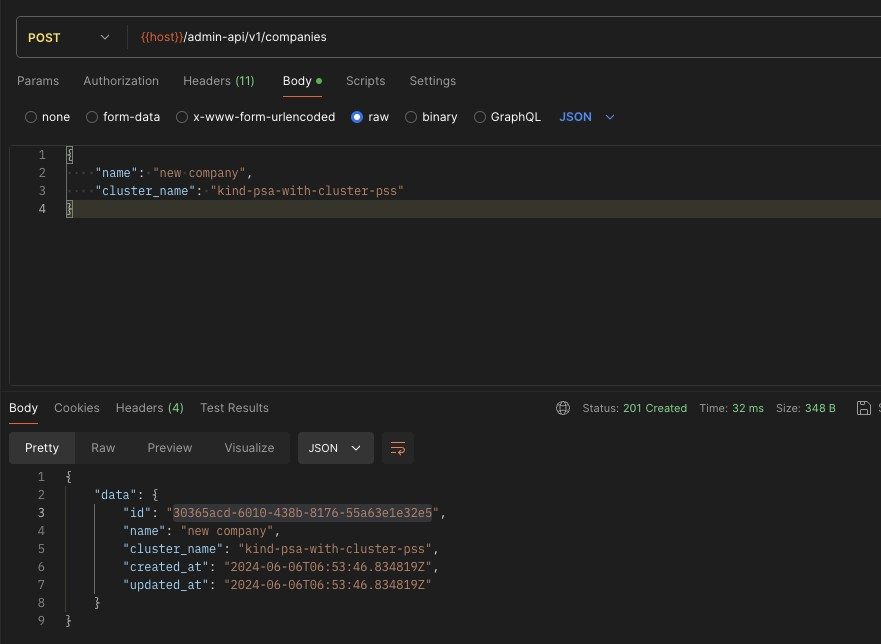
\includegraphics[width=0.8\textwidth]{resources/chapter-4/pengujian/p04-1.jpg}
  \caption{Pembuatan \textit{company} Untuk Pengujian P04}
  \label{fig:pengujian-p04-1}
\end{figure}


Admin menggunakan id company yang berhasil dibuat sesuai dengan gambar \ref{fig:pengujian-p04-1} sebagai parameter untuk \textit{company} yang dihapus. Berikut merupakan balikan dari \textit{request} yang dikirimkan.

\begin{figure}[ht]
  \centering
  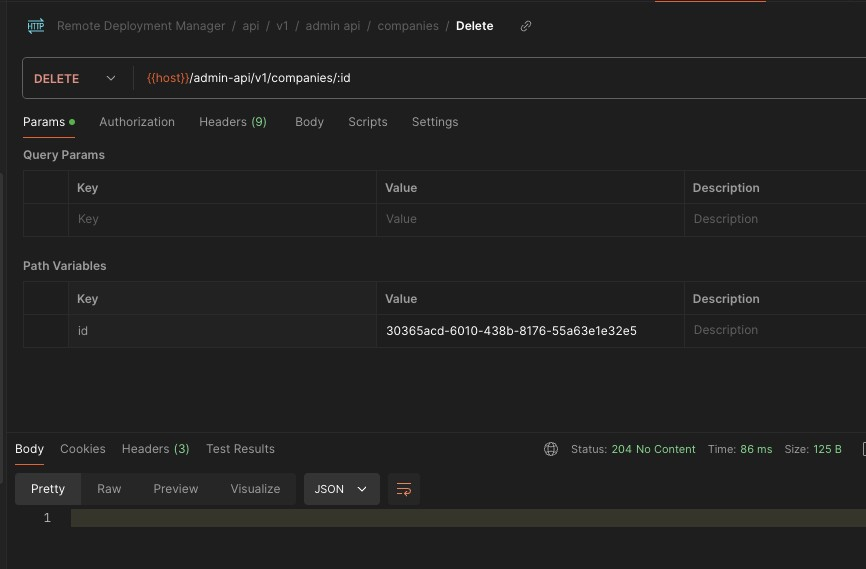
\includegraphics[width=0.8\textwidth]{resources/chapter-4/pengujian/p04.jpg}
  \caption{\textit{Request dan Response Pengujian} P04}
  \label{fig:pengujian-p04}
\end{figure}

Seluruh rekap pengujian pada domain \textit{company} dapat dilihat pada tabel \ref{tab:pengujian-domain-company}. Berdasarkan hasil yang diperoleh, terbukti bahwa kebutuhan fungsional dengan ID F01, F02, dan F03 telah terimplementasi dengan baik.


\bgroup
\begin{table}[ht]
  \def\arraystretch{1.5}
  \caption{Skenario dan Hasil Pengujian Domain \textit{Company}}
  \label{tab:pengujian-domain-company}
  \centering
  \begin{tabular}{|p{2cm}|p{2cm}|p{4cm}|p{3cm}|p{2cm}|}
    \hline
    \centering{ID Fungsional} & \centering{ID Pengujian} & \centering{Skenario}                                                                 & \centering{Ekspektasi}                                                                             & Realita \\
    \hline
    F01                       & P01                      & Admin mendaftarkan \textit{company} dengan cluster name yang tersedia                & Admin berhasil mendaftarkan \textit{company}                                                       & Sesuai  \\
    \hline
    F01                       & P02                      & Admin mendaftarkan \textit{company} dengan cluster name yang tidak valid             & Admin tidak berhasil mendaftarkan karena cluster name tidak valid                                  & Sesuai  \\
    \hline
    F02                       & P03                      & Admin membuat \textit{request} untuk melihat seluruh \textit{company} pada sistem    & Admin dapat melihat seluruh \textit{company} pada sistem                                           & Sesuai  \\
    \hline
    F03                       & P04                      & Admin melakukan DELETE \textit{request} untuk menghapus \textit{company} pada sistem & Admin dapat menghapus \textit{company} pada sistem dengan memberikan id company yang ingin dihapus & Sesuai  \\
    \hline
  \end{tabular}
\end{table}
\egroup


